%! TEX root = main.tex

\graphicspath{{00_Images/01_chapter/}}

\chapter{Introduction: Sound and Transducers}
\label{ch:sound_transducers}

\section{Course Context and The Nature of Sound}

Electroacoustics is the discipline that studies the mutual conversion between electrical signals and acoustic phenomena, with mechanical motion as the necessary physical intermediary. More precisely, the chain of transduction that underpins every audio system can be written as:
\[
\text{Electricity} \;\longleftrightarrow\; \text{Motion} \;\longleftrightarrow\; \text{Sound}
\]
The course takes the perspective of the full signal path: from the acoustic source, through the transducer that captures it, through all conditioning, amplification, and processing stages, and finally to the loudspeaker that reconstructs the sound field. This complete loop, from sound back to sound, motivates the systematic treatment of each physical domain and, crucially, the mathematical tools needed to pass between them.

\paragraph{John Tyndall and the foundations of acoustics} The first rigorous physical understanding of sound was established by a lineage of nineteenth-century natural philosophers whose work remains foundational. John Tyndall (1820-1893), Professor of Natural Philosophy at the Royal Institution of Great Britain from 1853 to 1887, devoted a celebrated series of eight public lectures to the subject, published in 1867 under the title Sound. Tyndall was an exceptional communicator of science and a pioneering alpinist who studied glaciers in the Alps; his name is commemorated in Tyndall Glaciers in Chile and Colorado, and in Mount Tyndall in California and Tasmania. His central experimental demonstration was the bell-in-vacuum experiment: a ringing bell suspended inside a sealed glass vessel gradually falls silent as air is evacuated from the chamber, proving unambiguously that sound requires a material medium for propagation. Light, by contrast, crosses the void of interplanetary space without difficulty; this contrast led Tyndall to distinguish what he called the world of sound, bounded by the presence of matter, from the wider universe accessible to light.

\paragraph{The World of Sound} This distinction was later crystallized by Sir William Henry Bragg (Nobel Prize in Physics, 1915) in his 1919 Christmas Lectures at the Royal Institution, published in 1920 as The World of Sound. The opening pages state that sound belongs to the world only: one may speak of the universe of light, but one can only speak of the world of sound. The implication for the engineer is direct: any acoustic transducer must operate within a material medium whose mechanical properties, density, compressibility, viscosity, govern both the propagation of sound and the efficiency of its generation.

\paragraph{What sound is, physically} Sound is not a substance but a motion: a mechanical disturbance that propagates through a continuous medium by transmitting momentum and energy from one layer of molecules to the adjacent one. In a gas such as air the disturbance takes the form of alternating compressions (regions of elevated pressure and density) and rarefactions (regions of reduced pressure and density) traveling outward from the source. The fundamental physical insight is that sound is the propagation of movement through the gas: no individual molecule travels from source to listener; instead, each molecule displaces its neighbour, and in this way the perturbation advances while the medium as a whole remains stationary on average.

\paragraph{Air as the acoustic medium} Air is a mixture of gases: approximately \(78\%\) nitrogen (\(\mathrm{N_2}\)), \(21\%\) oxygen (\(\mathrm{O_2}\)), about \(1\%\) argon (\(\mathrm{Ar}\)), and roughly \(0.04\%\) carbon dioxide (\(\mathrm{CO_2}\)), with traces of other species at the parts-per-million level. Despite being imperceptible to the touch, air carries a substantial mass: at \SI{20}{\degreeCelsius} and standard atmospheric pressure, the density of air is \(\rho_0 \approx \SI{1.2}{\kilo\gram\per\cubic\meter}\), meaning that one cubic meter of air weighs approximately \SI{1.2}{\kilo\gram}. This figure is far greater than intuition might suggest, and it is of primary physical importance: it is this inertia that any acoustic source must overcome in order to set the medium in motion, and it is also the physical origin of what will later be formalized as the acoustic mass, the distributed inertial load presented to a vibrating diaphragm by the surrounding air. The characteristic (specific) acoustic impedance of air at room temperature is:
\[
Z_0 = \rho_0 c \approx \SI{407}{\pascal\second\per\meter} \;\; [\text{Rayl}]
\]
where \(c \approx \SI{343}{\meter\per\second}\) is the adiabatic speed of sound. The unit of specific acoustic impedance, the Rayl, commemorates Lord Rayleigh (John William Strutt, 1842-1919), whose two-volume treatise The Theory of Sound (1877-1878) remains a cornerstone of acoustic science.

\section{The Electrodynamic Loudspeaker}

\subsection{Structure and Physical Components}

The electrodynamic loudspeaker is the most widespread acoustic transducer in use today. Its operating principle relies on the Lorentz force: a current-carrying conductor placed in a static magnetic field experiences a mechanical force proportional to the current. By placing a coil of wire in a strong, radially directed magnetic field and driving the coil with an audio-frequency current, the coil, together with the cone (diaphragm) rigidly attached to it, is set into oscillatory axial motion, which in turn radiates acoustic pressure waves into the surrounding air.
The principal physical components of a modern electrodynamic loudspeaker are as follows. The permanent magnet provides the static bias field; its flux is channeled through a soft-iron circuit comprising a pole piece, a front plate, and a rear plate, which together shape the field to be as uniform and radially directed as possible within the narrow air gap. The voice coil is a light cylindrical former wound with one or more layers of fine wire (typically aluminum or copper) and sits within the gap, carrying the signal current. The cone (diaphragm) is a stiff, light surface attached at its apex to the voice coil former and at its outer edge to the surround suspension; it converts the axial motion of the coil into acoustic radiation. The suspension (spider or damper) is a corrugated annular element that keeps the coil centered in the gap, provides the elastic restoring force that returns the diaphragm to rest when no signal is applied, and limits the axial displacement to safe values. The dust dome covers the open top of the voice coil former to prevent contamination of the gap.

\begin{figure}[!htb]
    \centering
    \subfloat[Cutaway photograph]{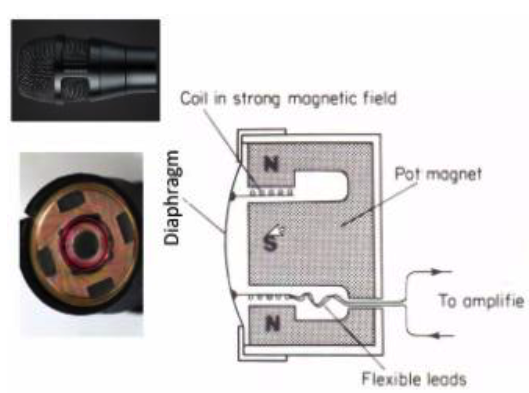
\includegraphics[height=0.2\textheight]{loudspeaker_cutaway.png}}
    \hfill
    \subfloat[Labeled cross-section]{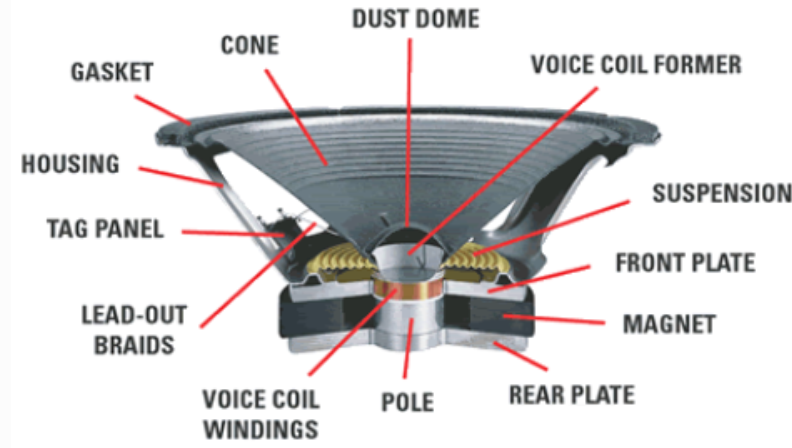
\includegraphics[height=0.2\textheight]{Loudspeaker_Structure.png}}
    \caption{An electrodynamic loudspeaker. The voice coil sits in the radial magnetic field formed between the pole piece and the front plate; the suspension and cone convert axial coil motion into acoustic radiation}
    \label{fig:loudspeakerStructure}
\end{figure}

\paragraph{Why the moving coil is called the voice coil} In the first generation of electrodynamic loudspeakers, permanent magnets powerful enough to produce a sufficiently intense gap field were not available. The static magnetic field was therefore generated by a second coil, wound directly on the magnetic circuit and energized by a DC supply, known as the field coil, because it produced the bias field rather than carrying the signal. The coil that carried the audio signal was distinguished from it by the name voice coil, signifying its role in reproducing the voice. With the advent of high-energy permanent-magnet materials (alnico in the 1930s, ferrite in the 1950s, neodymium in the 1980s), the field coil became obsolete; the name voice coil, however, was retained to designate the signal-carrying winding, and it remains in universal use in technical literature.

\subsection{The Lorentz Force on a Current-Carrying Conductor}

The fundamental law governing the electrodynamic transduction mechanism is the Lorentz force law. A point charge \(q\) moving with velocity \(\mathbf{u}\) in a magnetic field \(\mathbf{B}\) (measured in tesla, \(\si{\tesla} = \si{\newton\second\per\coulomb\per\meter}\)) experiences the vector force:
\[
\mathbf{F} = q \mathbf{u} \times \mathbf{B}
\]
The force is always perpendicular to both \(\mathbf{u}\) and \(\mathbf{B}\); its magnitude is:
\[
|\mathbf{F}| = q |\mathbf{u}| |\mathbf{B}| \sin\alpha
\]
where \(\alpha\) is the angle between the velocity of the charge and the field direction.

\begin{figure}[!htb]
    \centering
    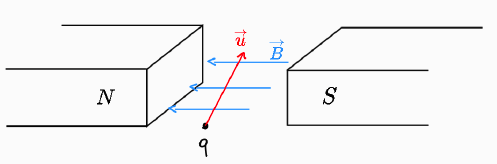
\includegraphics[width=0.50\linewidth]{lorentz_force.png}
    \caption{The Lorentz force on a positive charge \(q\) moving with velocity \(\mathbf{u}\) in a magnetic field \(\mathbf{B}\). The force \(\mathbf{F} = q \mathbf{u}\times\mathbf{B}\) is perpendicular to both vectors, with magnitude \(qu|\mathbf{B}|\sin\alpha\)}
\end{figure}

In a metallic conductor, many conduction electrons move simultaneously in response to an applied potential. For an infinitesimal volume element \(dV = S dl\) of a wire of cross-sectional area \(S\), the number of charge carriers is \(n dV\) (where \(n\) is the electron concentration per unit volume), and each contributes an infinitesimal Lorentz force:
\[
d\mathbf{F} = (-q \mathbf{u}\times\mathbf{B}) n dV
\]
Integrating over the full length \(L\) of the conductor:
\[
|\mathbf{F}| = n q |\mathbf{u}| |\mathbf{B}| \sin\alpha\cdot S L
\]
The electric current is the charge flowing per unit time: \(I = q n S |\mathbf{u}|\), so the expression simplifies to the compact motor law:

\begin{equation}
    |\mathbf{F}| = B l I \sin\alpha
    \label{eq:lorentzConductor}
\end{equation}

where \(l\) denotes the effective length of the wire in the field. In the loudspeaker, the voice coil is wound so that the current flow is perpendicular to the radial magnetic field at every point along the winding (\(\alpha = \pi/2\)), ensuring \(\sin\alpha = 1\) and, hence, the maximum possible force for a given current. Under this design condition, equation \eqref{eq:lorentzConductor} reduces to the fundamental motor law:
\[
F_C = B l i
\]

\begin{figure}[!htb]
    \centering
    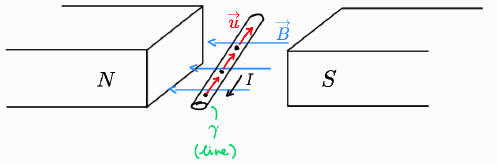
\includegraphics[width=0.50\linewidth]{wire_force.png}
    \caption{Infinitesimal wire element of cross-section \(S\) and length \(dl\) in a magnetic field \(\mathbf{B}\). Integrating the Lorentz force over the full winding length \(l\) yields the total axial force \(F_C = BlI\) when the current is perpendicular to the field}
\end{figure}

\subsection{Linearity and the Force Factor}

The product \(Bl\), called the force factor, with units \(\si{\newton\per\ampere} = \si{\tesla\meter}\), is the central electromagnetic parameter of the loudspeaker motor. The fundamental significance of the motor law \(F_C = Bl i\) lies in its linearity: if both \(B\) and \(l\) are constant throughout the voice coil's stroke, the driving force on the diaphragm is an exact linear replica of the driving current, with no additional harmonic or intermodulation content introduced at this stage of transduction. Conversely, any spatial variation of \(Bl\) with coil position, caused by inhomogeneities in the gap field, by flux modulation due to the signal current, or by the coil partially exiting the gap at large excursions, translates directly into harmonic and intermodulation distortion in the reproduced sound, degrading audio fidelity. The design of the magnetic circuit is therefore directed at maintaining the product \(Bl\) as spatially uniform as possible over the entire rated excursion of the voice coil.
The same Lorentz principle operates in the electrodynamic microphone, where the roles of force and motion are interchanged: acoustic pressure moves the diaphragm and the attached voice coil in the field, inducing a back-EMF proportional to the coil velocity, \(v = Bl u\), which constitutes the output electrical signal. The force factor \(Bl\) thus governs the transduction sensitivity in both directions, and maximizing it while maintaining spatial uniformity is common to both loudspeaker and microphone design.

\subsection{Electrical–Mechanical–Acoustical Conversion Chain}

The complete transduction path of a loudspeaker can be decomposed into three successive domain conversions, each governed by distinct physical laws:
\[
\text{Electrical}\;(v, i)
\;\longrightarrow\;
\text{Mechanical}\;(F, u)
\;\longrightarrow\;
\text{Acoustical}\;(P, U)
\]
At each interface the power variables of one domain are mapped to those of the next, while instantaneous power is conserved in the lossless idealization: electrical power \(P_E = v i\) becomes mechanical power \(P_M = F u\), which in turn becomes acoustic power \(P_A = P U\), where \(P\) is the acoustic pressure and \(U = u S_D\) is the volume velocity (the product of particle velocity and diaphragm area \(S_D\)). In practice, resistive losses in the voice coil (resistance \(R_{EC}\)), mechanical damping in the suspension (resistance \(R_{MS}\)), and the finite radiation resistance of the acoustic load all dissipate a fraction of the input power; a real loudspeaker typically converts less than \(2\%\) of the electrical input into radiated sound.

\begin{figure}[!htb]
    \centering
    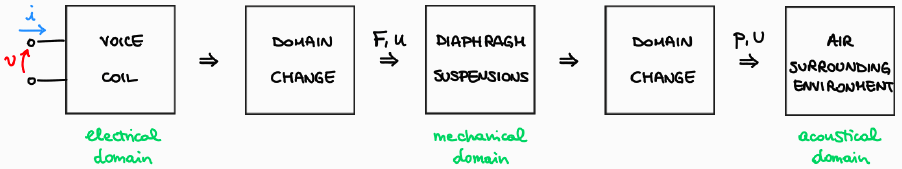
\includegraphics[width=0.75\textwidth]{conversion_chain.png}
    \caption{Block diagram of the loudspeaker transduction chain. Three physical domains are linked by two domain translations; each translation conserves instantaneous power (\(vi = Fu = PU\)) in the lossless idealization}
\end{figure}

The framework to be developed in the following chapter, the theory of electromechanical analogies, provides the mathematical tools for representing each domain and each domain translation as an equivalent electrical circuit element, so that the entire chain from electrical input to acoustic output can be analyzed with standard network-analysis methods.

\paragraph{Woofers and tweeters} The trade-off between moving mass, suspension compliance, and diaphragm area determines the usable frequency range of a driver. Woofers (low-frequency drivers) use large-area, relatively massive diaphragms to displace the air volume needed for efficient low-frequency radiation; tweeters (high-frequency drivers) use small, very light diaphragms so that the inertial reactance of the moving mass does not limit the response at high frequencies. These design constraints will be made quantitative once the full equivalent-circuit model of the loudspeaker is established in the chapters that follow.